\chapter{Experiments \& Results}\label{ch:results}

Given a parameterized framework for generating instances of resource exchanges,
experiments are designed and executed to explore the efficiency and quality of
solutions provided by different solvers. 

\S \ref{results:setup} describes the experimentation apparati, including the
computational tools, solvers and relevant output. Two experimental campaigns
were conducted. A scaling campaign, described in \S \ref{results:scale}, was
performed in order to investigate formulation behavior as a function of problem
size. \S \ref {results:stochastic} then describes the results of a stochastic
campaign.

\section{Experimental Setup}\label{results:setup}

An experiment consists of a set of resource-exchange graph instances executed
with a collection of configured solvers. When a solution is found, the solution
(i.e., the flow vector), the time required to reach the solution, and the
objective value (i.e., the dot-product of cost and flow vectors) are
recorded. Because solution time is a quantity of interest, all instances in an
experiment must be executed on homogeneous architecture. Furthermore, all
experiments must be executed on equivalent, homogeneous architecture in order to
quantify valid comparisons in solutions times across experimental campaigns.

Six execution nodes on UW-Madison Advanced Computing Initiative (ACI) HTCondor
system form the homogeneous environment used to conduct the experiments herein
described. Each execute node is comprised of an 2.90 GHz eight-core,
sixteen-thread, Intel Xeon E5-2690 \cite{intelproc} processor with 128 GB of
RAM. Processor hyper-threading was disabled for the duration of the experimental
campaign to allow comparisons between solution times.

For each experimental study, an input database consisting of persisted resource
exchange graph instances is generated. A copy of the database is transferred
from a user's submit node to each of the six execution nodes. A WorkQueue master
process is initiated. Sixteen workers per node are initialized using WorkQueue's
\texttt{condor\_submit\_workers} CLI. The master maintains a queue of instances
to be solved, assigning instances to workers as workers become available. Upon
completion, the input database is removed from each execution node, and the
results are collected from the user's submit node. The resulting database is
then post-processed and analyzed.

\subsection{Solvers and Formulations}

Three solvers are executed for each resource exchange graph instance: the Greedy
Heuristic, described in \S \ref{abm:dre:nfctp:heur}, COIN's LP solver
(COIN-CLP), and COIN's branch-and-cut solver (COIN-CBC). Each problem instance
is constructed as a \texttt{ExchangeGraph}, i.e., at the \textit{exchange layer}
shown in Figure \ref{fig:dre_impl} and Figure \ref{fig:dre_time}. The Greedy
Heuristic is applied directly to the \texttt{ExchangeGraph}. The CLP and CBC
solvers require a translation to the \textit{formulation layer}. The CLP solver
is applied to the LP formulation of the NFCTP and the CBC solver is applied to
the MILP formulation. The solution time, $t_s$ of a given solver is defined as
the time required to return a vector of arc flows given an
\texttt{ExchangeGraph} instance as shown in Figure \ref{fig:dre_time}.

\begin{equation}\label{eqn:solnt}
t_s = t_f - t_i
\end{equation}

\begin{figure}
  \begin{center}
    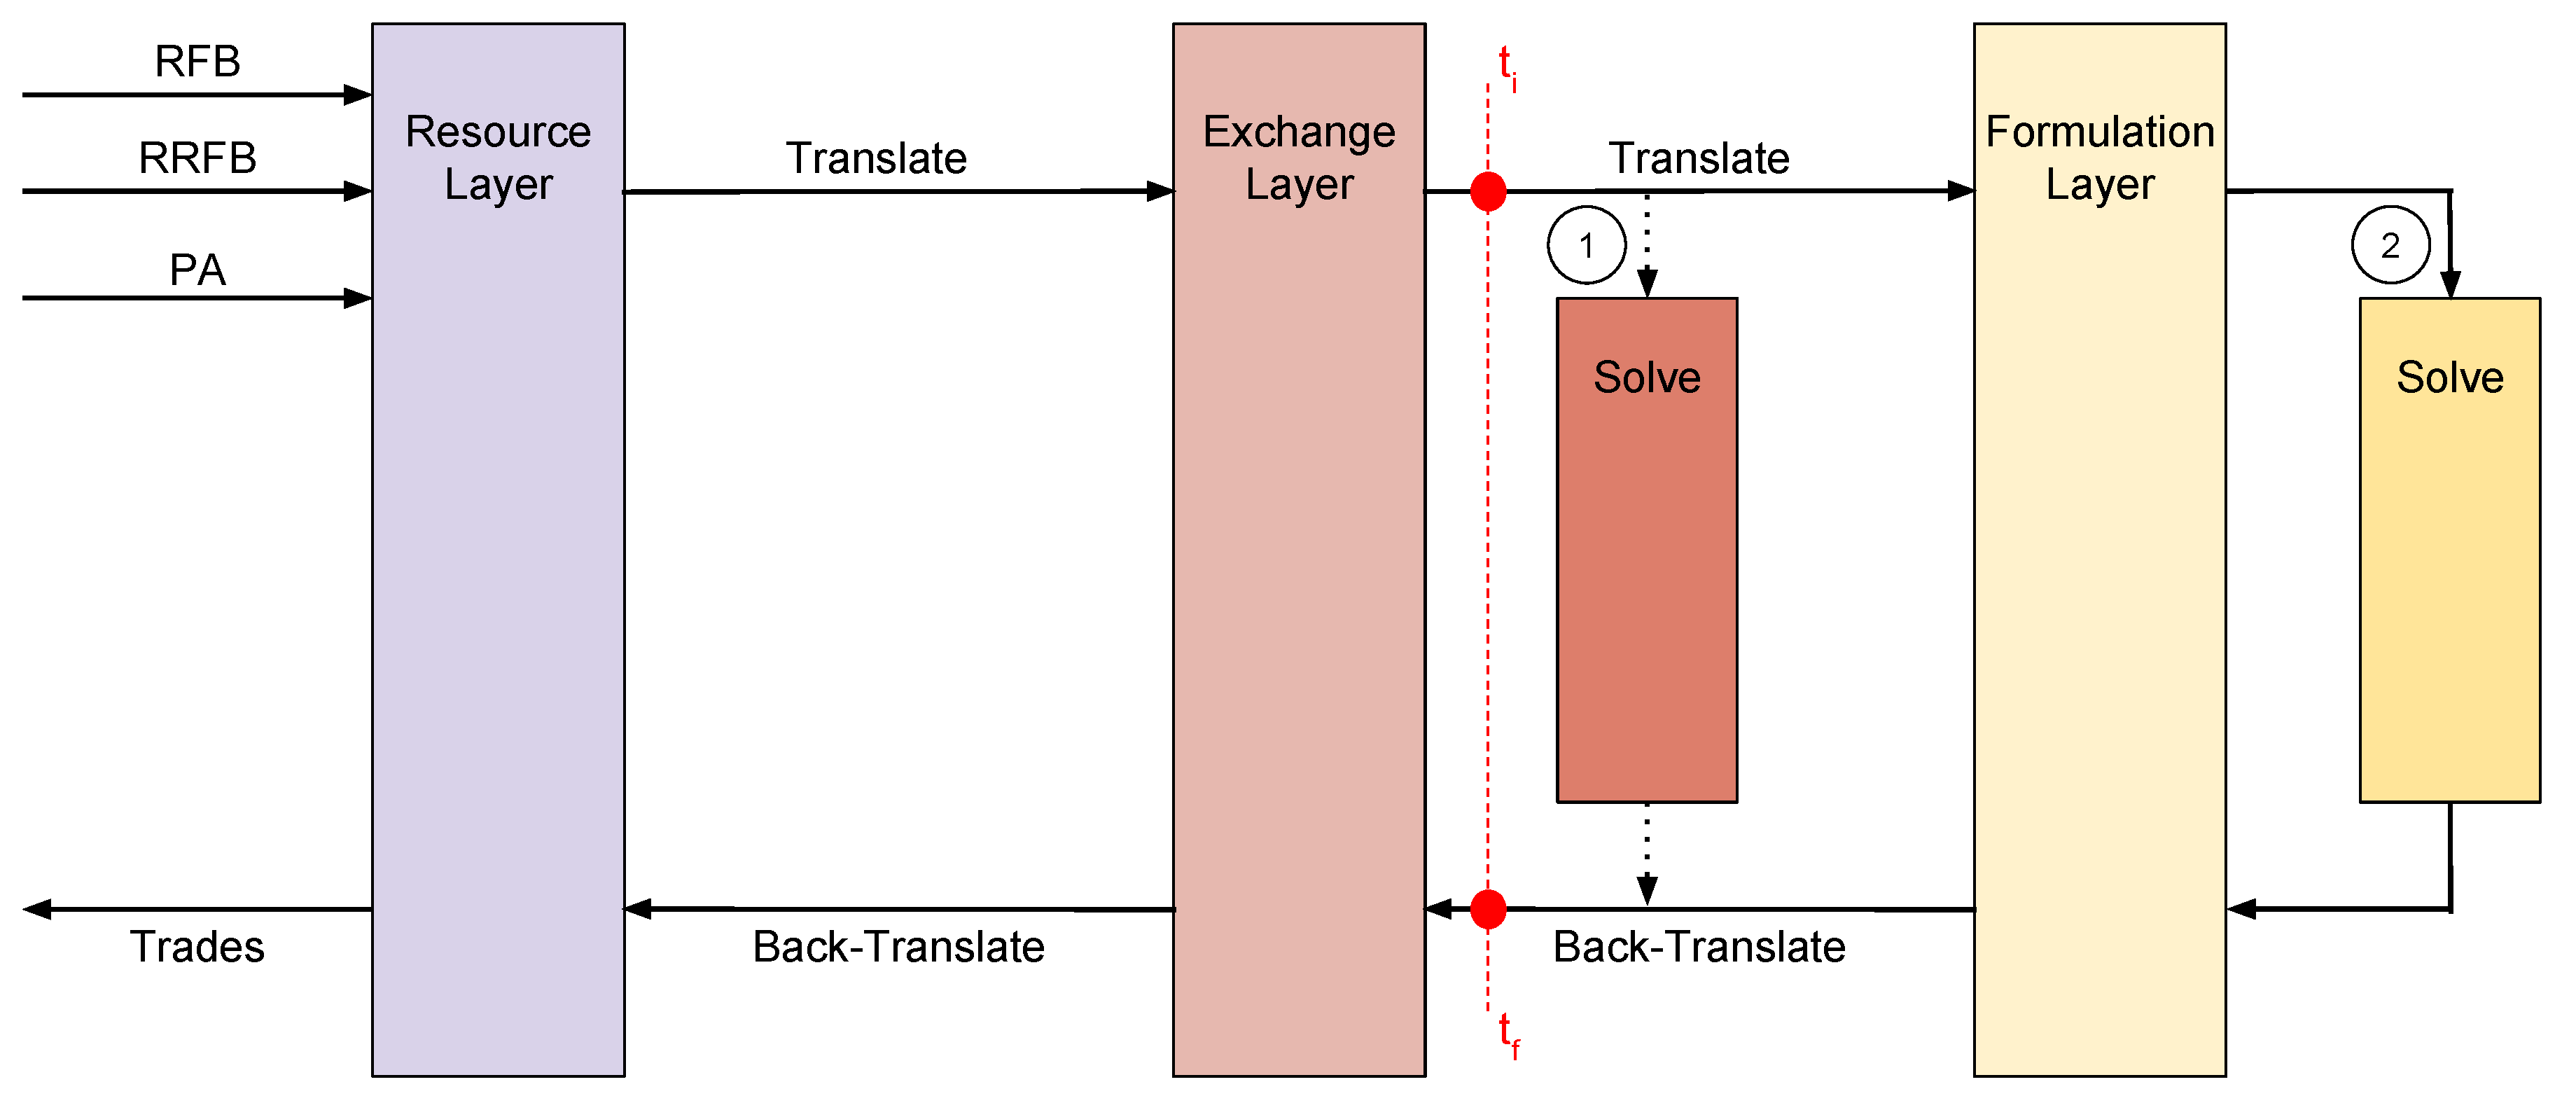
\includegraphics[width=\textwidth]{exchange_xlation_timing.pdf}
    \caption[]{
      \label{fig:dre_time}
      The time points for comparing different solutions using Equation \ref{eqn:solnt}.}
  \end{center}
\end{figure}

\TODO{Complexity of Greedy Solver, Translation}

\subsection{Parameter Variation}

\S \ref{method:setup:params} describes the parameters defining both Front and
Back-End exchanges. Each combination of fundamental parameters represents a
significant modeling assumption. Therefore, every experiment is conducted for
every combination of fundamental parameters: eighteen combinations in total. For
exchange types, a reference instance parameter vector is chosen. Experiments,
then, are conducted by perturbing instance parameter values from the reference
vector and comparing the output between a reference case and a perturbed case.

\subsubsection{Front-End Reference Instance Parameters}

\todo{Description of assumptions for each parameter}

\begin{table}[h!]
\centering
\caption{Reference Values for Front-End Exchange Instance Parameters.}
\label{tbl:front_ref_params}
\begin{tabular}{|c|c|}
\hline
Parameter    & Reference Value
\\ \hline
$r_{rx, \text{Th}}$   & 0.75 
\\ \hline
$r_{rx, \text{FThOX}}$ & 0.25
\\ \hline
$r_{l, c}$ & 1
\\ \hline
$f_{mox}$     & 0.33
\\ \hline
$r_{s, \text{Th}}$ & 0.08
\\ \hline
$r_{s, \text{TMOX}, \text{UOX}}$ & 1.
\\ \hline
$r_{s, \text{FMOX}}$ & 0.2
\\ \hline
$r_{s, \text{FThOX}}$ & 0.2
\\ \hline
$r_{inv, proc}$   & 1
\\ \hline
\end{tabular}
\end{table}


\subsubsection{Back-End Reference Instance Parameters}

\todo{Description of assumptions for each parameter}

\begin{table}[h!]
\centering
\caption{Reference Values for Back-End Exchange Instance Parameters.}
\label{tbl:back_ref_params}
\begin{tabular}{|c|c|}
\hline
Parameter    & Reference Value
\\ \hline
$r_{rx, \text{Th}}$   & 0.75 
\\ \hline
$r_{rx, \text{FThOX}}$ & 0.25
\\ \hline
$r_{l, c}$ & 1
\\ \hline
$f_{mox}$     & 0.33
\\ \hline
$r_{s, \text{Th}}$ & 0.08
\\ \hline
$r_{s, \text{TMOX}, \text{UOX}}$ & 1.
\\ \hline
$r_{s, \text{FMOX}}$ & 0.2
\\ \hline
$r_{s, \text{FThOX}}$ & 0.2
\\ \hline
$r_{s, \text{Repo}}$   & 0.2
\\ \hline
\end{tabular}
\end{table}

\subsection{Analysis Metrics}

The most obvious metrics to compare between solutions is the solution time,
$t_s$, and objective function value $z$,

\begin{equation}\label{eqn:obj_flow}
z = \sum_{(i, j) \in A} c_{i, j} x_{i, j}.
\end{equation}

However, while the objective function is minimized in the NFCTP formulations, it
necessarily includes flow along false arcs. Considering all arcs that exist both
in the formulation and the simulation, $A_{\text{sim}}$, another valid
comparison is dot product of preference and flow vectors. This value can be
considered the ``simulation objective'', i.e.,

\begin{equation}\label{eqn:sim_flow}
z_{\text{sim}} = \sum_{(i, j) \in A_{\text{sim}}} p_{i, j} x_{i, j}.
\end{equation}

The preference vector, $\vec{p}$, can be divided into its two components,
$\vec{p} = \vec{p}_c + \vec{p}_l$. If $f_{\text{loc}}$ is zero, then, by
definition, $\vec{p}_l = 0$, otherwise, it is comprised of non-zero
components. $\vec{p}_c$, however, is invariant under all values of
$f_{\text{loc}}$. Therefore, the commodity contribution of the simulation
objective, shown in Equation \ref{eqn:cpref_flow} is also an interesting
metric. It allows for direct investigation of the effect of adding
location-based preferences to the system. Furthermore, comparisons can be made
between systems with coarse and fine location-based preferences using this
metric.

\begin{equation}\label{eqn:cpref_flow}
z^c_{\text{sim}} = \sum_{(i, j) \in A_{\text{sim}}} p^c_{i, j} x_{i, j}.
\end{equation}

Each of the above metrics compare aggregate values between solutions. That is,
comparisons are being made at a macroscopic scope. For any two solutions to
identical problem instances, though, more detailed comparisons can be made. The
individual flow values, and values derived therefrom, can be compared directly
using a well-known normative measure. In order to compare values across problem
sizes, the root mean square (RMS), related to the $L_2$ norm, is used to measure
the microscopic differences between two solution values. The RMS analysis can be
applied to any flow-related metric for two solutions, $\vec{x}^1$ and
$\vec{x}^2$. Equation \ref{eqn:rms_flow} shows the equation for the flow RMS,
and Equation \ref{eqn:rms_pref} displays the commodity-preference flow RMS.

\begin{equation}\label{eqn:rms_flow}
RMS_{\text{flow}} = \sqrt{ \frac{1}{N} \sum_i (x^1_i - x^2_i) ^2 }
\end{equation}

\begin{equation}\label{eqn:rms_pref}
RMS_{\text{pref}} = \sqrt{ \frac{1}{N} \sum_i {p_i^c}^2 (x^1_i - x^2_i)^2 }
\end{equation}

\section{Scalability Campaign}\label{results:scale}

\subsection{Front-End Exchanges}

\subsubsection{Reference Case}
% Include large and small

\subsubsection{Instance Parameter Variation}
% Include large and small r_l_c

\subsubsection{Convergence Criteria}

\subsection{Back-End Exchanges}

\subsubsection{Reference Case}
% Include large and small

\subsubsection{Instance Parameter Variation}
% Include large and small r_l_c

\subsubsection{Convergence Criteria}

\section{Stochastic Campaign}\label{results:stochastic}

\subsection{Front-End Exchanges}
% talk about base parameter vector

\subsubsection{Fundamental Parameter Variation}

\subsubsection{Instance Parameter Variation}

\subsection{Back-End Exchanges}
% talk about base parameter vector

\subsubsection{Fundamental Parameter Variation}

\subsubsection{Instance Parameter Variation}

\section{Observations}
